\documentclass[titlepage, 12pt]{article}
\usepackage[utf8]{inputenc}
\usepackage{multirow}

\usepackage[english,serbian]{babel}
\usepackage{graphicx}

\begin{document}

\title{Dejvid Anderson}
\author{Ilić Branko \\ 216/2018 \\mi18216@alas.matf.bg.ac.rs \and  Niketić Anđela \\ 109/2018 \\ mi18109@alas.matf.bg.ac.rs\and Lukić Mila \\ 222/2018 \\mi18222@alas.matf.bg.ac.rs\and Kučinar Veljko \\ 144/2018 \\ mi18144@alas.matf.bg.ac.rs}
\date{\today}

\maketitle
\tableofcontents
\section{Uvod}

\begin{tabular}{|c|c|c|}
\hline
\multicolumn{2}{|c|}{Dejvid Poup Anderson}\\
\hline
\multicolumn{2}{|c|}{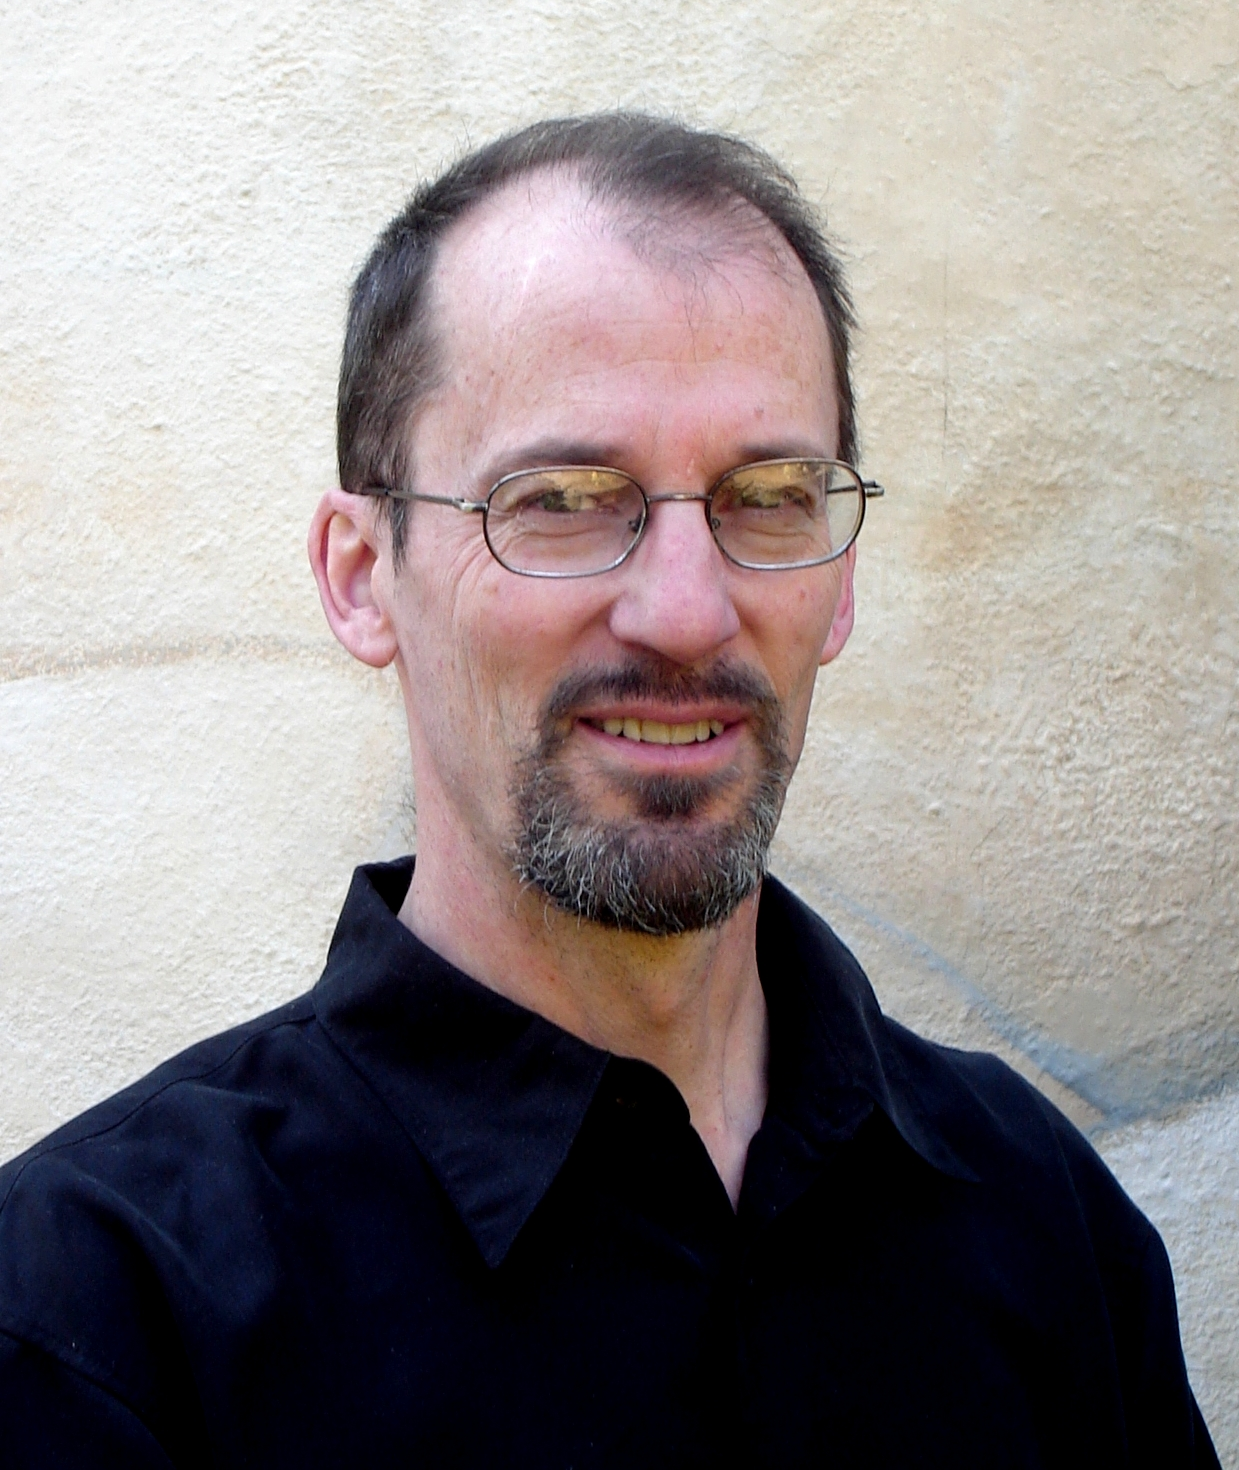
\includegraphics[width=220px,height=261px]{dejvid.jpg}}\\

\hline
Ime po rođenju & Dejvid Poup Anderson \\
\hline
Datum rođenja & 1955.(63/64 god)\\
\hline
Mesto rođenja & Oukland(Kalifornija), SAD\\
\hline
Prebivalište & Berkli(Kalifornija)\\
\hline
\multirow{2}{*}{Obrazovanje}&Univerzitet Veslijan\\
&Univerzitet Viskonsin-Medison\\
\hline 
Zanimanje & Informatika\\
\hline
Delovanje & Volontersko računanje \\
\hline
\multirow{2}{*}{Nagrade}&NSF Presidential Young Investigator Award\\
&IBM Faculty Development Grant
\\
\hline
\end{tabular}
\\
\\
\newline

Dejvid Poup Anderson je američki istraživač u Laboratoriji za Svemirske Nauke (engl. Space Sciences Laboratory - SSL), na kalifornijskom Univerzitetu u Berkliju (engl. University of California, Berkeley), kao i vanredni profesor kompjuterskih nauka na Univerzitetu u Hjustonu (engl. University of Houston). Anderson takođe vodi i SETI@home, BOINC, BOSSA i Bolt softverske projekte.
\subsection{Edukacija}
Anderson je završio osnovne akademske studije iz matematike na Univerzitetu Veslijan(engl. Wesleyan University) i iz informatike na Univerzitetu Viskonsin-Medison(engl. University of Wisconsin-Madison). Tokom master-studija, objavio je četiri istraživačka rada koja su se bavila računarskom grafikom[1]. Njegov doktorski rad bavio se korišćenjem gramatika sa poboljšanim atributima zarad bližeg određivanja i implementacije komunikacionih protokola.

\subsection{Karijera}
Od 1985. do 1992. godine bio je asistent na kalifornijskom Univerzitetu u Berkliju u odeljku za kompjuterske nauke, gde je dobio Presidential Young Investigator nagradu od strane Nacionalne Fondacije za Nauku(engl. National Science Foundation) i Faculty Development nagradu od strane IBM-a. Tokom ovog perioda vodio je nekoliko istraživačkih projekata:
\begin{description}
	\item[FORMULA] (Forth Music Language), programski jezik i rantajm sistem za ekspresivnu računarsku muziku baziran na Forth-u.
	\item[MOOD] (Musical Object-Oriented Dialect), paralelni programski jezik i rantajm sistem za računarsku muziku baziran na C++.
	
	\item[DASH], distribuirani operativni sistem sa podrškom za digitalni audio i video.
	
	\item[Continuous Media File System] (CMFS), sistem datoteka za digitalni audio i video.
	
	\item[Comet], U/I server za digitalni audio i video.
	
\end{description}
Od 1992. do 1994. godine, Anderson je radio za kompaniju Sonic Solutions, gde je razvio Sonic System, prvi distribuirani sistem za profesionalno editovanje digitalnog audio sadržaja.

\subsubsection{Izumi}
Godine 1994. izumeo je "Virtual Reality Television", televizijski sistem koji je dozvoljavao korisnicima da upravljaju njihovom virtuelnom pozicijom i orijentacijom. Nagrađen je patentom za ovaj izum 1996. godine.

Godine 1994. je razvio jedan od prvih sistema za kolaborativno filtriranje(engl. collaborative filtering), i razvio veb-sajt rare.com, koji je davao predloge za filmove u odnosu na ocene korisnika.

Od 1995. do 1998. godine bio je tehnički direktor(engl. Chief Technical Officer) Tunes.com-a, gde je razvio sistem baziran na Veb-u za pronalazak muzike zasnovan na kolaborativnom filtriranju, akustike, i drugim modelima.

Godine 1995. pridružio se Dejvidu Gediju(engl. David Gedye) i Denu Vertimeru(engl. Dan Werthimer) da bi kreirali SETI@home, tek osnovan volonterski kompjuterski projekat. Anderson nastavlja da upravlja SETI@home.

Od 2000. do 2002. godine bio je glavni tehnološki direktor(engl. Chief Technology Officer) United Devices-a, kompanije koja je razvijala softver za raspodeljeno izračunavanje.

\subsubsection{Berkli Otvorena Infrastruktura za mrežno računanje}
Godine 2002. osnovao je projekat Berkli Otvorenu Infrastrukturu za mrežno računanje (engl. Berkeley Open Infrastructure for Network Computing - BOINC) koji razvija platformu za softver otvorenog koda za volontersko računanje (engl. Volunteer Computing). Projekat je finansiran od strane Nacionalne Fondacije za Nauku (engl. National Science Foundation) i sedište se nalazi u laboratiriji za svemirske nauke (engl. Space Science Laboratories), na kalifornijskom Univerzitetu u Berkliju. BOINC koristi oko 100 projekata, uključujući i SETI@home, Einstein@home, Rosetta@home, Climateprediction.net, kao i IBM World Community Grid. Koristi se kao platforma za distribuirane aplikacije na poljima kao što su matematika, medicina, molekularna biologija, klimatologija, i astrofizika.

Anderson je bio uključen i u projekat Stardust@home, u kom je učestvovalo 23,000 volontera koji su u slikama na Veb-u tražili međuzvezdane čestice prašine - pristup koji se naziva podeljeno razmišljanje (engl. distributed thinking). Godine 2007, Anderson je pokrenuo dva nova softverska projekta: BOSSA (posredni softver za podeljeno razmišljanje) i Bolt (platforma za obuku baziranu na Veb-u i edukaciju u kontekstu volonterskog računanja ili podeljenog razmišljanja).

\subsubsection{Berkli otvoreni sistem za prikupljanje veština}
Berkli otvoreni sistem za prikupljanje veština(engl. The Berkeley Open System for Skill Aggregation - BOSSA) je softverska platforma za podeljeno razmišljanje(engl. distributed thinking), koristi volontere na Internetu za ispunjavanje zadataka koji zahtevaju ljudsku inteligenciju, znanje, ili veštine prepoznavanja.

\newpage
\begin{thebibliography}{9}
\bibitem{referenca1}
  
  \textit{„Hidden Line Elimination in Projected Grid Surfaces”},
\bibitem{referenca2}
    \textit{„Formula: a programming language for expressive computer music”},
\bibitem{referenca3}
    \textit{ „The DASH Project: An Overview | EECS at UC Berkeley”},
    www2.eecs.berkeley.edu
\bibitem{referenca4}
    \textit{ „A File System for Continuous Media”},
\bibitem{referenca5}
    \textit{„A Continuous Media I/O Server and its Synchronization Mechanism”},
\bibitem{referenca6}
    Anderson, D.; Doris, R.; Moorer, J.
    \textit{ „A Distributed Computer System for Professional Audio”},
    New York, USA,
    1994.
\bibitem{refrenca7}
    \textit{„U.S. Patent 5,714,997: Virtual Reality Television System”},
\bibitem{refrenca8}
    \textit{BOINC - Berkeley Open Infrastructure for Network Computing},
\bibitem{refrenca9}
    \textit{ „Wayback Machine”},
    web.archive.org. 2012-03-06. 
\end{thebibliography}

\end{document}
